\documentclass[12pt, a4paper]{article}

\renewcommand{\figurename}{Figura}

\usepackage[
  outputdir=target,
  newfloat=true
]{minted}
\SetupFloatingEnvironment{listing}{name=Código}

\usepackage{indentfirst}
\usepackage{graphicx}

\title{Trabalho Prático 4}
\author{Bernardo Ferrari \and Matheus Teixeira}
\date{Novembro 2019}

\begin{document}
\maketitle

\section{Introdução}

Esse trabalho propõem uma solução para a simulação de estacionamento de
caminhões utilizando a biblioteca \textbf{jFuzzy} juntamente a um cliente
java conectado a simulação através de sockets.

\section{Desenvolvimento}

Foi desenvolvido um programa cliente em java que recebe a posição $(x, y)$, $x, y \in [0, 1]$,
acompanhada do angulo $angle \in [0, 360]$ entre o caminhão e o fundo do estacionamento.
É feita a computação da direção do volante do caminhão como saída $wheel \in [-1.0, 1.0]$.

Essa computação é feita através de um sistema fuzzy descrito em `Fuzzy Control Language' (FCL) e
essa descrição é interpretada pela biblioteca java jFuzzy e para executar as computações é executado
o código java~\ref{listing:jfuzzy}.

\begin{listing}[h!]
  \begin{minted}[breaklines]{java}
String fileName = "src/driver.fcl";
FIS fis = FIS.load(fileName,true);
fis.setVariable("x_pos", x);
fis.setVariable("angle", angle);
fis.evaluate();
double respostaDaSuaLogica = fis.getVariable("wheel").getValue();
  \end{minted}
  \caption{Utilização da biblioteca jFuzzy.}\label{listing:jfuzzy}
\end{listing}

Note que o código~\ref{listing:jfuzzy} lê de um arquivo chamado \textbf{driver.fcl}.
Esse arquivo descreve em FCL o comportamento do sistema fuzzy e inclui as definições
de variáveis de entrada e de saída, definições de \textit{fuzzify} das variáveis de entrada,
definições de \textit{defuzzify} das variáveis de saída e as definições das regras fuzzy.

Para o \textit{fuzzify} da variável $x\_pos$, foram criados conjuntos fuzzy para $center$, $left$ e $right$ utilizando trapézios para definição probabilidades.
Os conjuntos fuzzy para a variável $x\_pos$ são descritos pelo bloco fuzzify descritos no código~\ref{listing:xposfuzzy} e na figura~\ref{figure:xposfuzzy}.

\begin{listing}[h!]
  \begin{minted}[breaklines]{text}
FUZZIFY x_pos
  TERM center := TRAPE 0.0 0.2 0.8 1.0;
  TERM left := TRAPE -0.1 0 0.2 0.5;
  TERM right := TRAPE 0.5 0.8 1 1.1;
END_FUZZIFY
\end{minted}
  \caption{Conjuntos fuzzy para variável de entrada $x\_pos$.}\label{listing:xposfuzzy}
\end{listing}

\begin{figure}[h!]
  \centering
  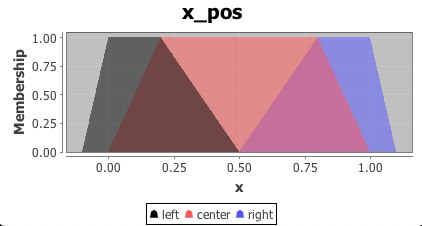
\includegraphics[width=0.8\textwidth]{assets/x_pos.jpg}
  \caption{Conjuntos fuzzy para variável de entrada $x\_pos$.}\label{figure:xposfuzzy}
\end{figure}

Para o \textit{fuzzify} da variável $angle$, foram criados conjuntos fuzzy para $up$, $right$, $left$ e $down$ com sobreposição entre os trapézios.
Além de $up\_left$, $left\_down$, $down\_right$ e $right\_up$, para melhor controle das regiões de intersecção dos conjuntos $up$, $right$, $left$ e $down$.
Os conjuntos fuzzy para a variável $angle$ são descritos pelo bloco fuzzify descritos no código~\ref{listing:anglefuzzy} e na figura~\ref{figure:anglefuzzy}.

\begin{listing}[h!]
  \begin{minted}[breaklines]{text}
FUZZIFY angle
  TERM up         := TRAPE 0 80 100 180;
  TERM up_left    := TRAPE 90 120 150 180;
  TERM left       := TRAPE 90 170 190 270;
  TERM left_down  := TRAPE 180 210 240 270;
  TERM down       := TRAPE 180 260 280 360;
  TERM down_right := TRAPE 270 300 330 360;
  TERM right      := (0, 1) (2.5, 1) (90, 0) (270, 0) (357.5, 1) (360, 1);
  TERM right_up   := TRAPE 0 30 60 90;
END_FUZZIFY
  \end{minted}
  \caption{Conjuntos fuzzy para variável de entrada $angle$.}\label{listing:anglefuzzy}
\end{listing}

\begin{figure}[h!]
  \centering
  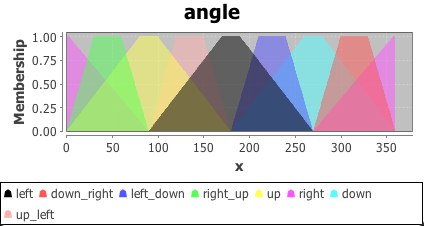
\includegraphics[width=0.8\textwidth]{assets/angle.jpg}
  \caption{Conjuntos fuzzy para variável de entrada $angle$.}\label{figure:anglefuzzy}
\end{figure}

Para o \textit{defuzzify} da variável de saída $wheel$, foram criados conjuntos para $straight$, $turn\_left$ e $turn\_right$ com sobreposição entre os trapézios.
Foi usado o método de centro de gravidade COG para defuzzificação da variável de valor padrão $default = 0$.
Os conjuntos fuzzy para a variável $wheel$ são descritos pelo bloco defuzzify descritos no código~\ref{listing:wheelfuzzy} e na figura~\ref{figure:wheelfuzzy}.

\begin{listing}[h!]
  \begin{minted}[breaklines]{text}
DEFUZZIFY wheel
  TERM straight := TRAPE -0.5 -0.1 0.1 0.5;
  TERM turn_left := TRAPE -1.1 -1 -0.5 0;
  TERM turn_right := TRAPE 0 0.5 1 1.1;
  METHOD : COG;
  DEFAULT := 0;
END_DEFUZZIFY
  \end{minted}
  \caption{Conjuntos fuzzy para variável de saída $wheel$.}\label{listing:wheelfuzzy}
\end{listing}

\begin{figure}[h!]
  \centering
  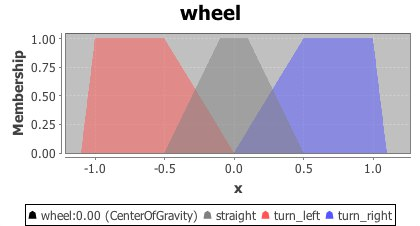
\includegraphics[width=0.8\textwidth]{assets/wheel.jpg}
  \caption{Conjuntos fuzzy para variável de entrada $wheel$.}\label{figure:wheelfuzzy}
\end{figure}

As regras foram descritas de maneira a refletir a intuição de um motorista de caminhão ao estacionar.
Para isso foram criadas vinte e quatro regras, sendo resultado de uma regra para cada conjunto fuzzy de $x\_pos$ em combinação com cada conjunto fuzzy de $angle$ sendo $3 \times 8 = 24$.

Quanto o caminhão se encontra no conjunto $left$ ou no conjunto $right$ ele possui uma tendencia fazer a variável $wheel$ virar o volante com o objetivo de convergir a variável $x\_pos$ para o conjunto $center$.
Já quando se $x\_pos$ se encontra no conjunto $center$, o objetivo das regras é mantes o caminhão no conjunto $center$.
Assim fazendo com que o caminhão sempre se alinhe com $x\_pos = 0.5$.

Para controlar a convergência da posição $y$, as cardinalidades $left\_down$ e $down\_right$ fazem com que a variavel $wheel$ vire o caminhão para descer o caminhão até o estacionamento.

As descrições das regras se encontram no apêndice~\ref{sec:apendice}


\section{Conclusão}

\appendix
\section{Regras do sistema fuzzy}\label{sec:apendice}

\begin{minted}[breaklines]{text}
RULEBLOCK drive
  // Use 'min' for 'and' (also implicit use 'max'
  // for 'or' to fulfill DeMorgan's Law)
  AND : MIN;
  // Use 'min' activation method
  ACT : MIN;
  // Use 'max' accumulation method
  ACCU : MAX;

  RULE 1 : IF x_pos IS left AND angle IS right      THEN wheel IS turn_right;
  RULE 2 : IF x_pos IS left AND angle IS right_up   THEN wheel IS turn_right;
  RULE 3 : IF x_pos IS left AND angle IS up         THEN wheel IS turn_right;
  RULE 4 : IF x_pos IS left AND angle IS up_left    THEN wheel IS straight;
  RULE 5 : IF x_pos IS left AND angle IS left       THEN wheel IS straight;
  RULE 6 : IF x_pos IS left AND angle IS left_down  THEN wheel IS turn_left;
  RULE 7 : IF x_pos IS left AND angle IS down       THEN wheel IS turn_left;
  RULE 8 : IF x_pos IS left AND angle IS down_right THEN wheel IS turn_left;

  RULE 9  : IF x_pos IS right AND angle IS right      THEN wheel IS straight;
  RULE 10 : IF x_pos IS right AND angle IS right_up   THEN wheel IS straight;
  RULE 11 : IF x_pos IS right AND angle IS up         THEN wheel IS turn_left;
  RULE 12 : IF x_pos IS right AND angle IS up_left    THEN wheel IS turn_left;
  RULE 13 : IF x_pos IS right AND angle IS left       THEN wheel IS turn_left;
  RULE 14 : IF x_pos IS right AND angle IS left_down  THEN wheel IS turn_right;
  RULE 15 : IF x_pos IS right AND angle IS down       THEN wheel IS turn_right;
  RULE 16 : IF x_pos IS right AND angle IS down_right THEN wheel IS turn_right;

  RULE 17 : IF x_pos IS center AND angle IS right      THEN wheel IS turn_right;
  RULE 18 : IF x_pos IS center AND angle IS right_up   THEN wheel IS turn_right;
  RULE 19 : IF x_pos IS center AND angle IS up         THEN wheel IS straight;
  RULE 20 : IF x_pos IS center AND angle IS up_left    THEN wheel IS turn_left;
  RULE 21 : IF x_pos IS center AND angle IS left       THEN wheel IS turn_left;
  RULE 22 : IF x_pos IS center AND angle IS left_down  THEN wheel IS turn_left;
  RULE 23 : IF x_pos IS center AND angle IS down       THEN wheel IS turn_left;
  RULE 24 : IF x_pos IS center AND angle IS down_right THEN wheel IS turn_right;

END_RULEBLOCK
\end{minted}

\end{document}
